\documentclass[11pt,a4paper]{article}

\usepackage[margin=2.4cm]{geometry}
\usepackage{iftex}
\ifPDFTeX
  \usepackage[T1]{fontenc}
  \usepackage[utf8]{inputenc}
  \usepackage{tgpagella}
  \usepackage{tgheros}
\else
  \usepackage{fontspec}
  \setmainfont{TeX Gyre Pagella}
  \setsansfont{TeX Gyre Heros}
\fi
\usepackage[serbian]{babel}
\usepackage{microtype}
\usepackage{booktabs}
\usepackage{tabularx}
\usepackage{array}
\usepackage{amsmath}
\usepackage{amssymb}
\usepackage{graphicx}
\usepackage{xcolor}
\usepackage{hyperref}
\usepackage{enumitem}
\usepackage{caption}
\usepackage{float}
\usepackage{pdfpages}

\addto\captionsserbian{%
  \renewcommand{\abstractname}{Abstract}%
}

\graphicspath{{report_figures/}}
\hypersetup{
  colorlinks=true,
  linkcolor=blue!45!black,
  urlcolor=blue!55!black,
  citecolor=blue!45!black,
  pdftitle={Učenje podsticanjem u BipedalWalker okruženju},
  pdfauthor={Aleksa Mojsić}
}
\setlist{nosep}
\renewcommand{\arraystretch}{1.18}
\newcolumntype{Y}{>{\raggedright\arraybackslash}X}

\title{\textbf{Učenje podsticanjem u okruženjima\\
BipedalWalker-v3 i BipedalWalkerHardcore-v3}\\[0.5em]
\large Poređenje PPO, SAC i TD3 algoritama i razvoj SAC--LSTM pristupa}
\author{Aleksa Mojsić}
\date{\today}

\begin{document}

\maketitle

\begin{abstract}
U radu su ispitani algoritmi PPO, SAC i TD3 za upravljanje dvonožnim robotom
u okruženjima \texttt{BipedalWalker-v3} i
\texttt{BipedalWalkerHardcore-v3}. Standardne implementacije algoritama
korišćene su kao polazni modeli, dok je za zahtevniju varijantu razvijen
SAC agent koji koristi istoriju opservacija, LSTM mrežu i mehanizam za
sprečavanje stagnacije. Na standardnom zadatku najbolji prijavljeni srednji
rezultat postiže TD3 (\(299{,}54\)), dok PPO i TD3 u sprovedenim
eksperimentima nisu uspešno rešili hardcore varijantu. Najbolja sačuvana
višeepizodna evaluacija SAC--LSTM modela ostvaruje srednju sirovu nagradu
\(216{,}84\pm76{,}06\) u pet epizoda. Dobijeni rezultati pokazuju značajno
poboljšanje u odnosu na polazne modele, ali velika varijansa i trening sa
jednim glavnim semenom ne omogućavaju zaključak da je zahtevniji zadatak
stabilno rešen.
\end{abstract}

\newpage
\tableofcontents
\newpage

\section{Uvod i cilj projekta}

Učenje podsticanjem posmatra interakciju agenta i okruženja kao niz
odluka. Agent na osnovu stanja bira akciju, okruženje vraća nagradu i
novo stanje, a cilj je maksimizacija očekivane diskontovane sume nagrada
\begin{equation}
  G_t=\sum_{k=0}^{T-t}\gamma^k r_{t+k},
\end{equation}
gde je \(\gamma\in[0,1]\) faktor diskontovanja.

Cilj projekta je:
\begin{enumerate}
  \item poređenje PPO, SAC i TD3 algoritama na standardnom zadatku;
  \item ispitivanje prenosa tih pristupa na zahtevniji hardcore zadatak;
  \item razvoj sekvencijalnog modela koji koristi istoriju opservacija;
  \item analiza uticaja mehanizma za sprečavanje stagnacije na ponašanje agenta.
\end{enumerate}

Glavno istraživačko pitanje glasi: \emph{da li istorija opservacija, LSTM
mreža i eksplicitno kažnjavanje stagnacije mogu da poboljšaju ponašanje
agenta na okruženju \texttt{BipedalWalkerHardcore-v3}?}

\section{Okruženje i podaci}

Za razliku od nadgledanog učenja, u ovom problemu ne postoji unapred
pripremljen skup označenih primera. Podaci za obuku nastaju tokom
interakcije agenta sa Gymnasium okruženjem. Svaka tranzicija ima oblik
\[
  (s_t,a_t,r_t,s_{t+1},d_t),
\]
gde su \(s_t\) stanje, \(a_t\) akcija, \(r_t\) nagrada, a \(d_t\)
indikator završetka epizode. Tranzicije off-policy algoritama čuvaju se
u replay buffer-u i uzorkuju tokom treninga.

\subsection{Stanja i percepcije}

Opservacija je vektor od 24 realne vrednosti. Sadrži ugao i brzine tela,
položaje i ugaone brzine zglobova, kontakte nogu sa podlogom i deset
lidar merenja terena. Agent ne dobija sliku niti apsolutne koordinate.
U razvijenom pristupu poslednjih 12 opservacija formira sekvencu dimenzije
\(12\times24\).

\subsection{Akcije}

Akcioni prostor je kontinualan četvorodimenzioni vektor iz intervala
\([-1,1]^4\). Komponente određuju upravljanje motorima oba kuka i oba
kolena. Izlaz actor mreže se ograničava na dozvoljeni interval pre
prosleđivanja simulatoru.

\subsection{Nagrada i terminalna stanja}

Pozitivna nagrada podstiče kretanje udesno, dok se potrošnja obrtnog
momenta blago kažnjava. Kontakt trupa sa tlom donosi kaznu od \(-100\).
Epizoda se završava padom ili dolaskom do kraja staze, dok se pri
dostizanju vremenskog ograničenja prekida. Prema dokumentaciji,
standardna varijanta se smatra rešenom sa 300 poena u najviše 1600
koraka, a hardcore varijanta sa 300 poena u najviše 2000 koraka
\cite{gymnasium}.

Hardcore varijanta uvodi dodatne prepreke, poput merdevina, panjeva i
jama. Zbog složenijeg terena uvedena je kratka istorija opservacija, kako
bi model pri izboru akcije imao informaciju o neposredno prethodnom
kretanju i kontaktu sa preprekom.
Slika~\ref{fig:environment-comparison} prikazuje determinističke početne
kadrove oba okruženja za isto seme. Opservacija, pored prikazanog stanja
robota i terena, sadrži deset numeričkih lidar merenja.

\begin{figure}[H]
\centering
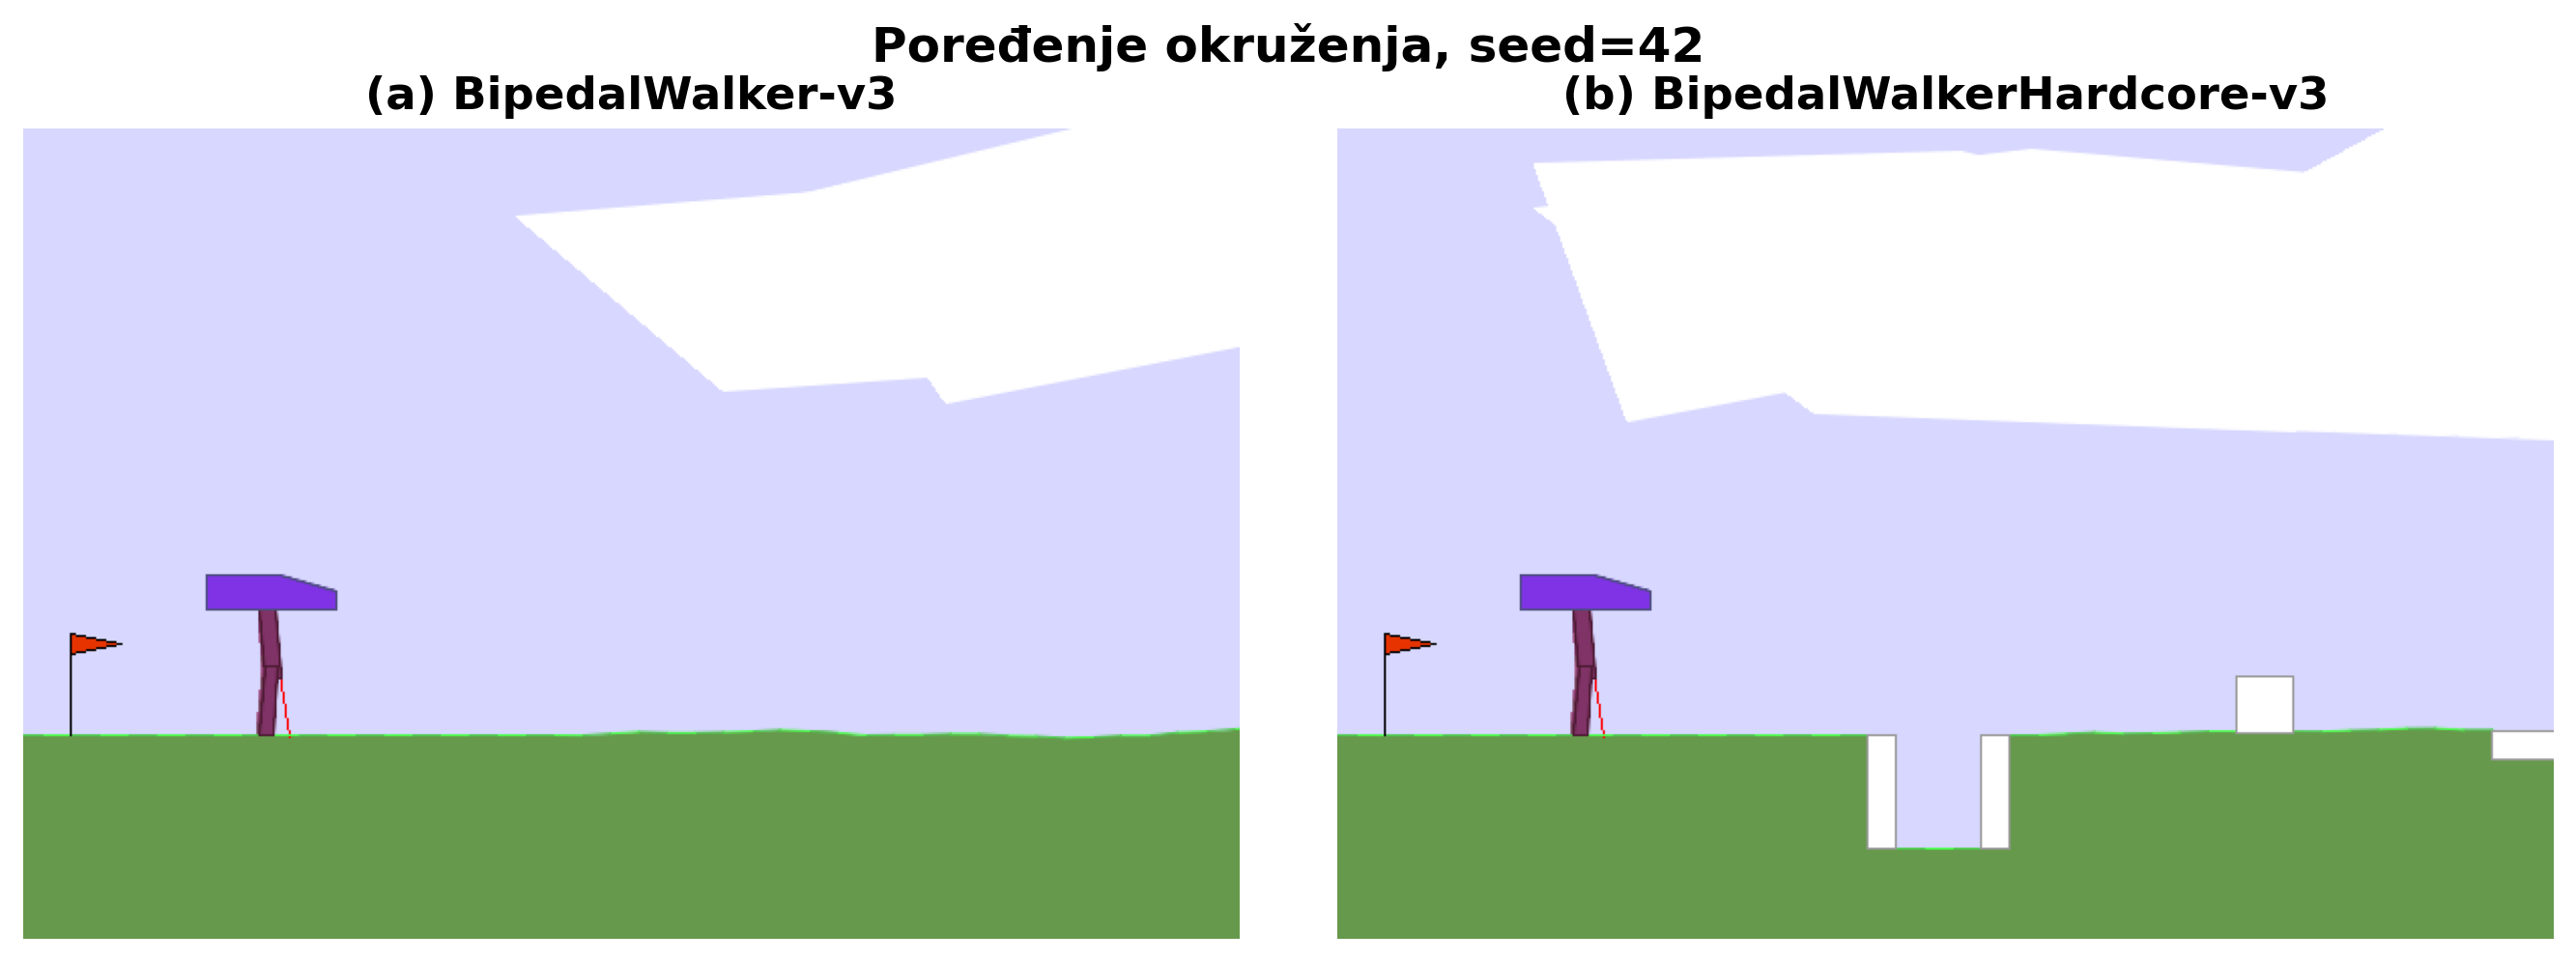
\includegraphics[width=\textwidth]{environment_comparison.png}
\caption{Poređenje standardnog okruženja \texttt{BipedalWalker-v3} i
zahtevnijeg okruženja \texttt{BipedalWalkerHardcore-v3}, koje uvodi
prepreke poput panjeva, jama i merdevina. Kadrovi su generisani direktno
iz Gymnasium okruženja sa semenom 42.}
\label{fig:environment-comparison}
\end{figure}

\section{Modeli}

\subsection{Polazni modeli}

Nasumična politika predstavlja najjednostavniji oblik upravljanja i služi
kao donja referentna vrednost. Njena sačuvana evaluacija na hardcore
okruženju iznosi \(-109{,}56\pm8{,}08\) u pet epizoda. Kao polazni modeli
korišćene su i standardne implementacije PPO, SAC i TD3 algoritama iz
biblioteke Stable-Baselines3 \cite{sb3}.

PPO je on-policy metod koji više puta optimizuje ograničenu surrogate
funkciju nad prikupljenim batch-em \cite{ppo}. SAC je off-policy
actor--critic metod koji, pored očekivane nagrade, maksimizuje entropiju
politike \cite{sac}. TD3 smanjuje precenjivanje Q-vrednosti korišćenjem
dva critic modela, zakašnjelih actor ažuriranja i izglađivanja ciljne
politike \cite{td3}.

\subsection{SAC--LSTM model}

Razvijeni model koristi niz od 12 uzastopnih opservacija. Sekvenca se
obrađuje LSTM enkoderom, a dobijena reprezentacija koristi se u actor i
critic mrežama.
SAC actor daje parametre stohastičke politike, dok dva critic modela
aproksimiraju \(Q(s,a)\). Ciljna vrednost je
\begin{equation}
 y=r+\gamma(1-d)\left[
 \min_{i\in\{1,2\}}Q_i'(s',a')-\alpha\log\pi(a'|s')
 \right].
\end{equation}
Actor se optimizuje tako da istovremeno bira akcije velike procenjene
vrednosti i održava istraživanje:
\begin{equation}
 J_\pi=\mathbb{E}\left[
 \alpha\log\pi(a|s)-\min_i Q_i(s,a)
 \right].
\end{equation}

Tok odluke prikazan je na Slici~\ref{fig:architecture}. Actor bira akciju
pri izvršavanju politike, dok se critic modeli i replay buffer koriste
tokom treninga.

\begin{figure}[H]
\centering
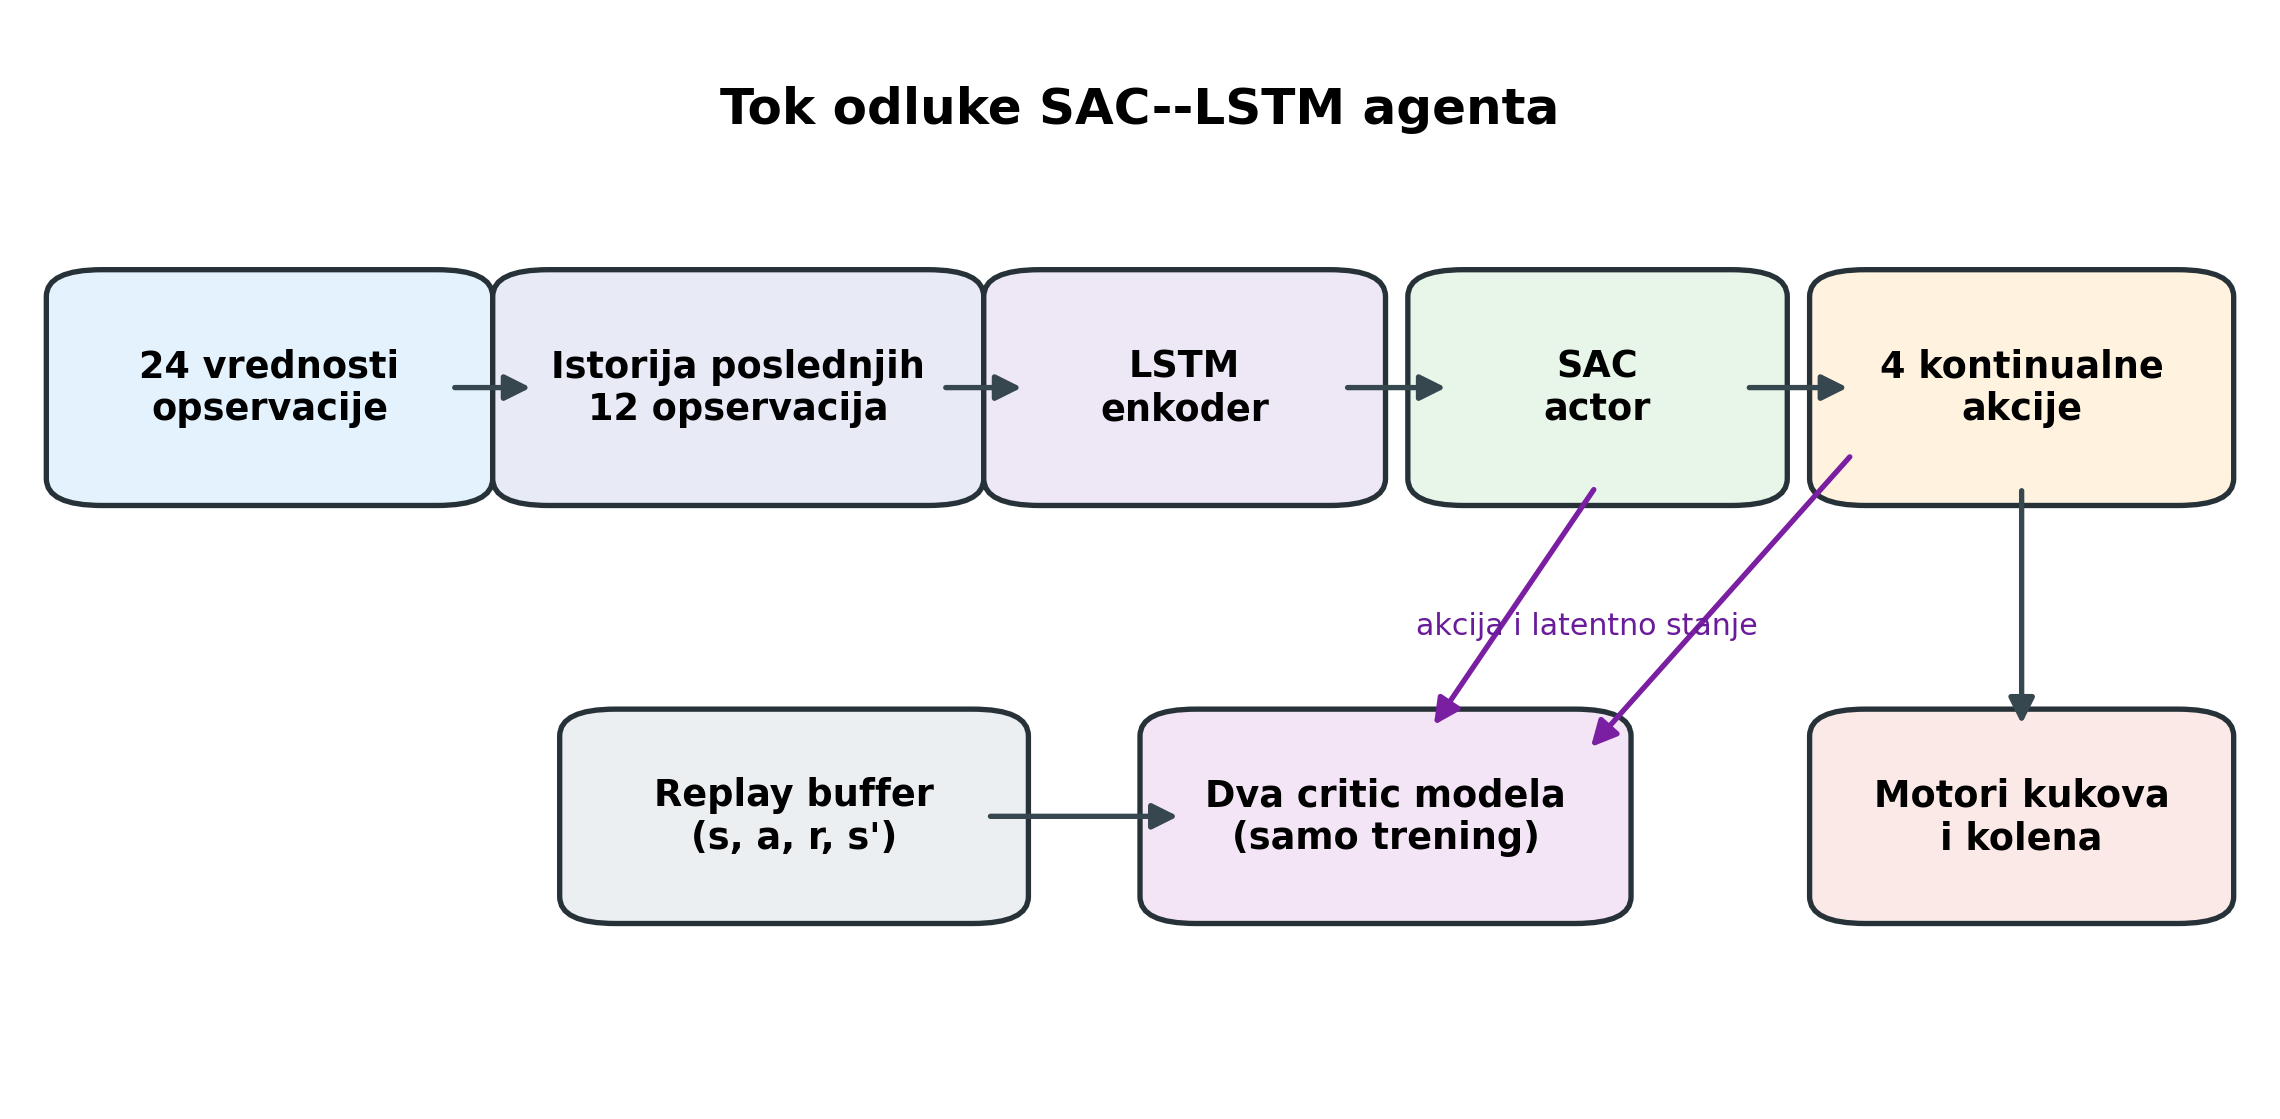
\includegraphics[width=\textwidth]{observation_action_diagram.png}
\caption{Poslednjih 12 opservacija, od kojih svaka ima 24 vrednosti,
obrađuje LSTM enkoder. SAC actor zatim proizvodi četiri kontinualne
akcije za motore kukova i kolena; dva critic modela učestvuju u
treningu.}
\label{fig:architecture}
\end{figure}

\subsection{Mehanizam za sprečavanje stagnacije}

Tokom ranih eksperimenata primećeno je da agent može dugo ostati
uspravan bez stvarnog napretka. Zbog toga je uveden dodatni mehanizam
koji prati horizontalni pomeraj u definisanom vremenskom prozoru. Nakon
početnog perioda bez provere, stagnacija se kažnjava, a posle zadatog
broja uzastopnih detekcija epizoda se prekida. Izmenjena funkcija nagrade
koristi se isključivo tokom treninga, dok se za konačno poređenje
prijavljuje originalna, sirova nagrada okruženja.

\section{Eksperimentalni protokol}

Implementacija koristi Python, Gymnasium, Stable-Baselines3, NumPy i
PyTorch. U glavnim eksperimentima korišćeno je seme 42. Pri evaluaciji se
koristi deterministička akcija modela, dok se početna semena okruženja
menjaju između epizoda. Standardni eksperimenti imaju 300\,000 koraka
treninga i pet evaluacionih epizoda. SAC--LSTM model koristi istoriju
dužine 12, \texttt{frame\_skip}=2 i periodično čuvanje najboljih stanja
modela.

Srednja vrednost i standardna devijacija nagrade računaju se kao
\[
 \bar r=\frac{1}{n}\sum_{i=1}^{n}r_i,\qquad
 \sigma_r=\sqrt{\frac{1}{n}\sum_{i=1}^{n}(r_i-\bar r)^2}.
\]


\section{Rezultati}

\subsection{Standardno okruženje}

\begin{table}[H]
\centering
\caption{Prijavljeni rezultati na \texttt{BipedalWalker-v3}, 300\,000
koraka, seme 42 i pet evaluacionih epizoda.}
\label{tab:standard}
\begin{tabular}{lrrr}
\toprule
Algoritam & Srednja nagrada & Std. dev. & Srednja dužina \\
\midrule
PPO & 125,28 & 131,29 & 989,6 \\
SAC & 282,08 & 0,91 & 1181,6 \\
TD3 & \textbf{299,54} & \textbf{0,46} & 797,0 \\
\bottomrule
\end{tabular}
\end{table}

TD3 ostvaruje najveću srednju nagradu i najmanju standardnu devijaciju,
SAC postiže visok i ujednačen rezultat, dok PPO pokazuje znatno veću
varijabilnost. Slika~\ref{fig:standard-rewards} poredi ove rezultate sa
SB3 referentnim modelima i javnim prijavama iz Hugging Face skupa
leaderboard rezultata \cite{hfleaderboard}. Rangovi na slici izračunati su
samo prema srednjoj nagradi, pa predstavljaju orijentaciono, a ne strogo
kontrolisano poređenje.

\begin{figure}[H]
\centering
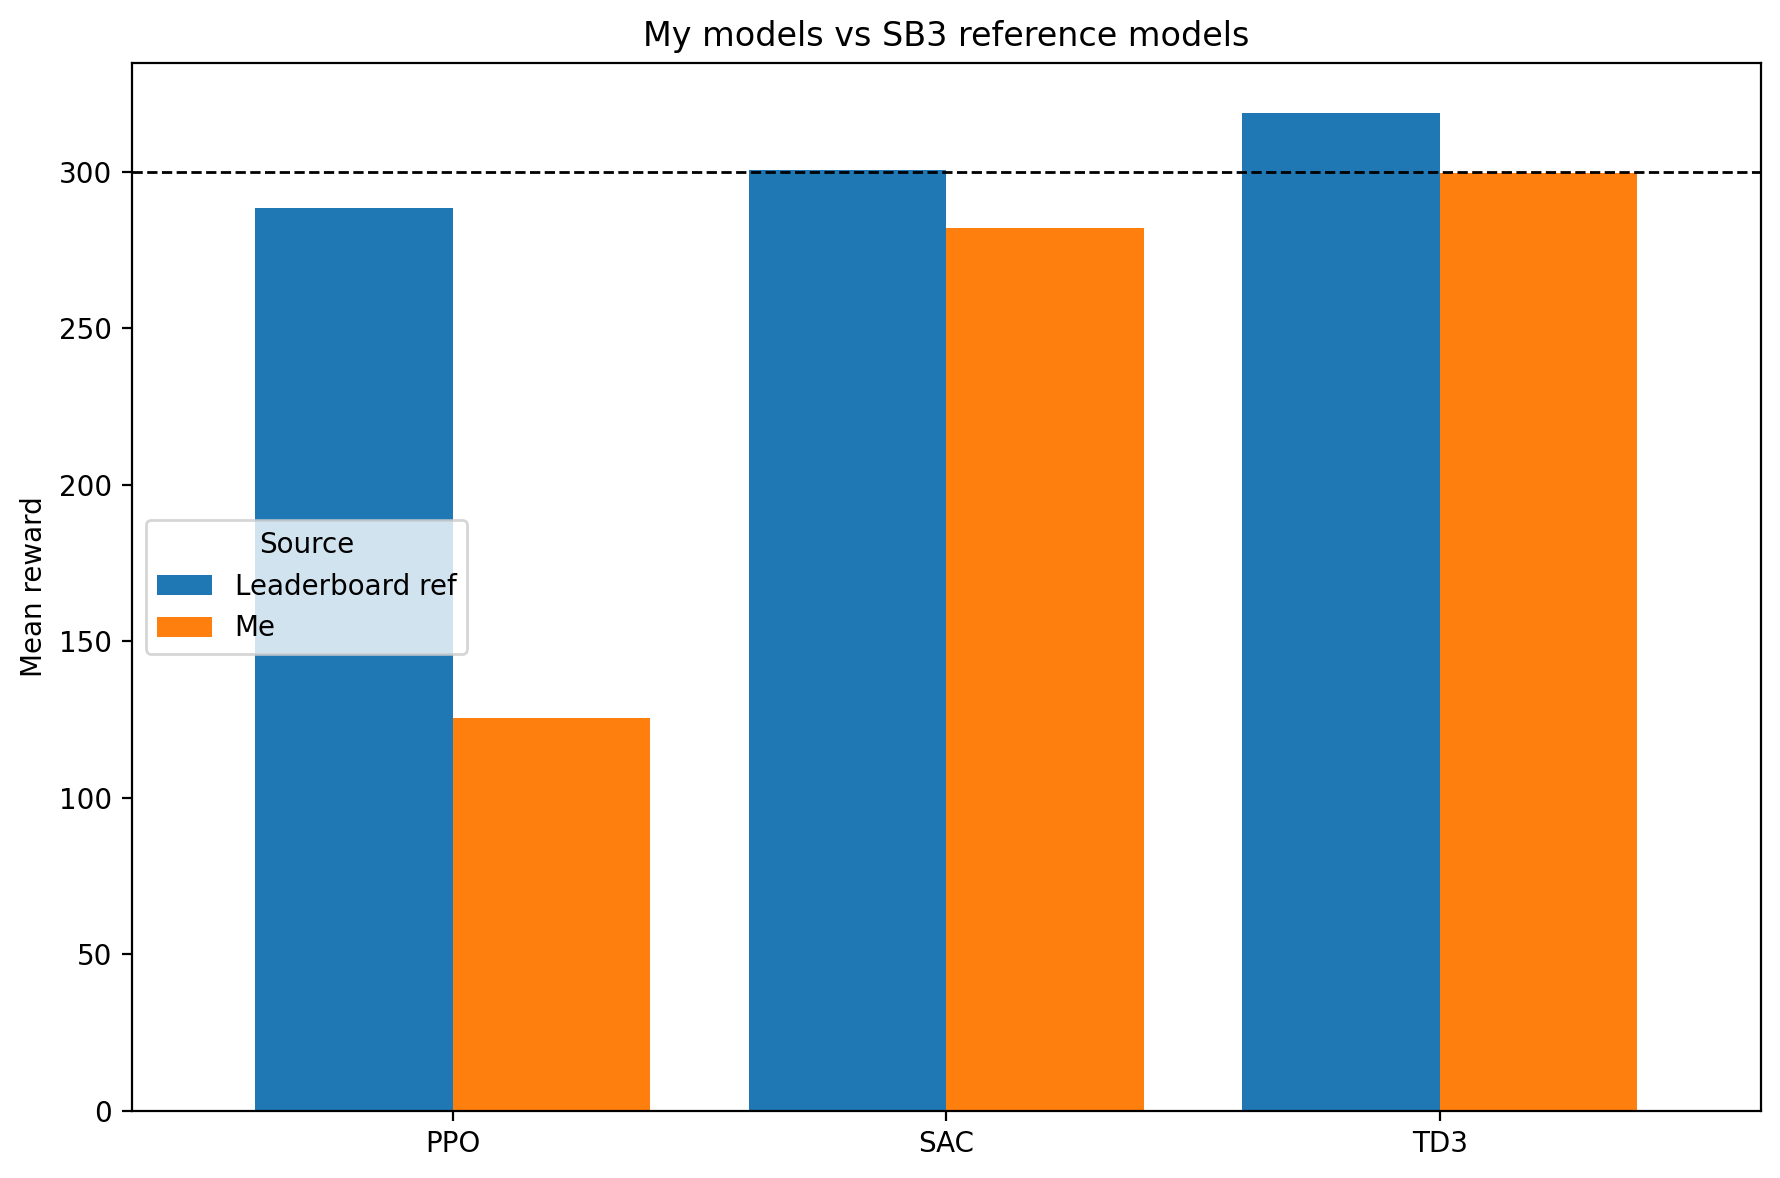
\includegraphics[width=.69\textwidth]{bipedalwalker_me_vs_sb3_refs.png}

\medskip
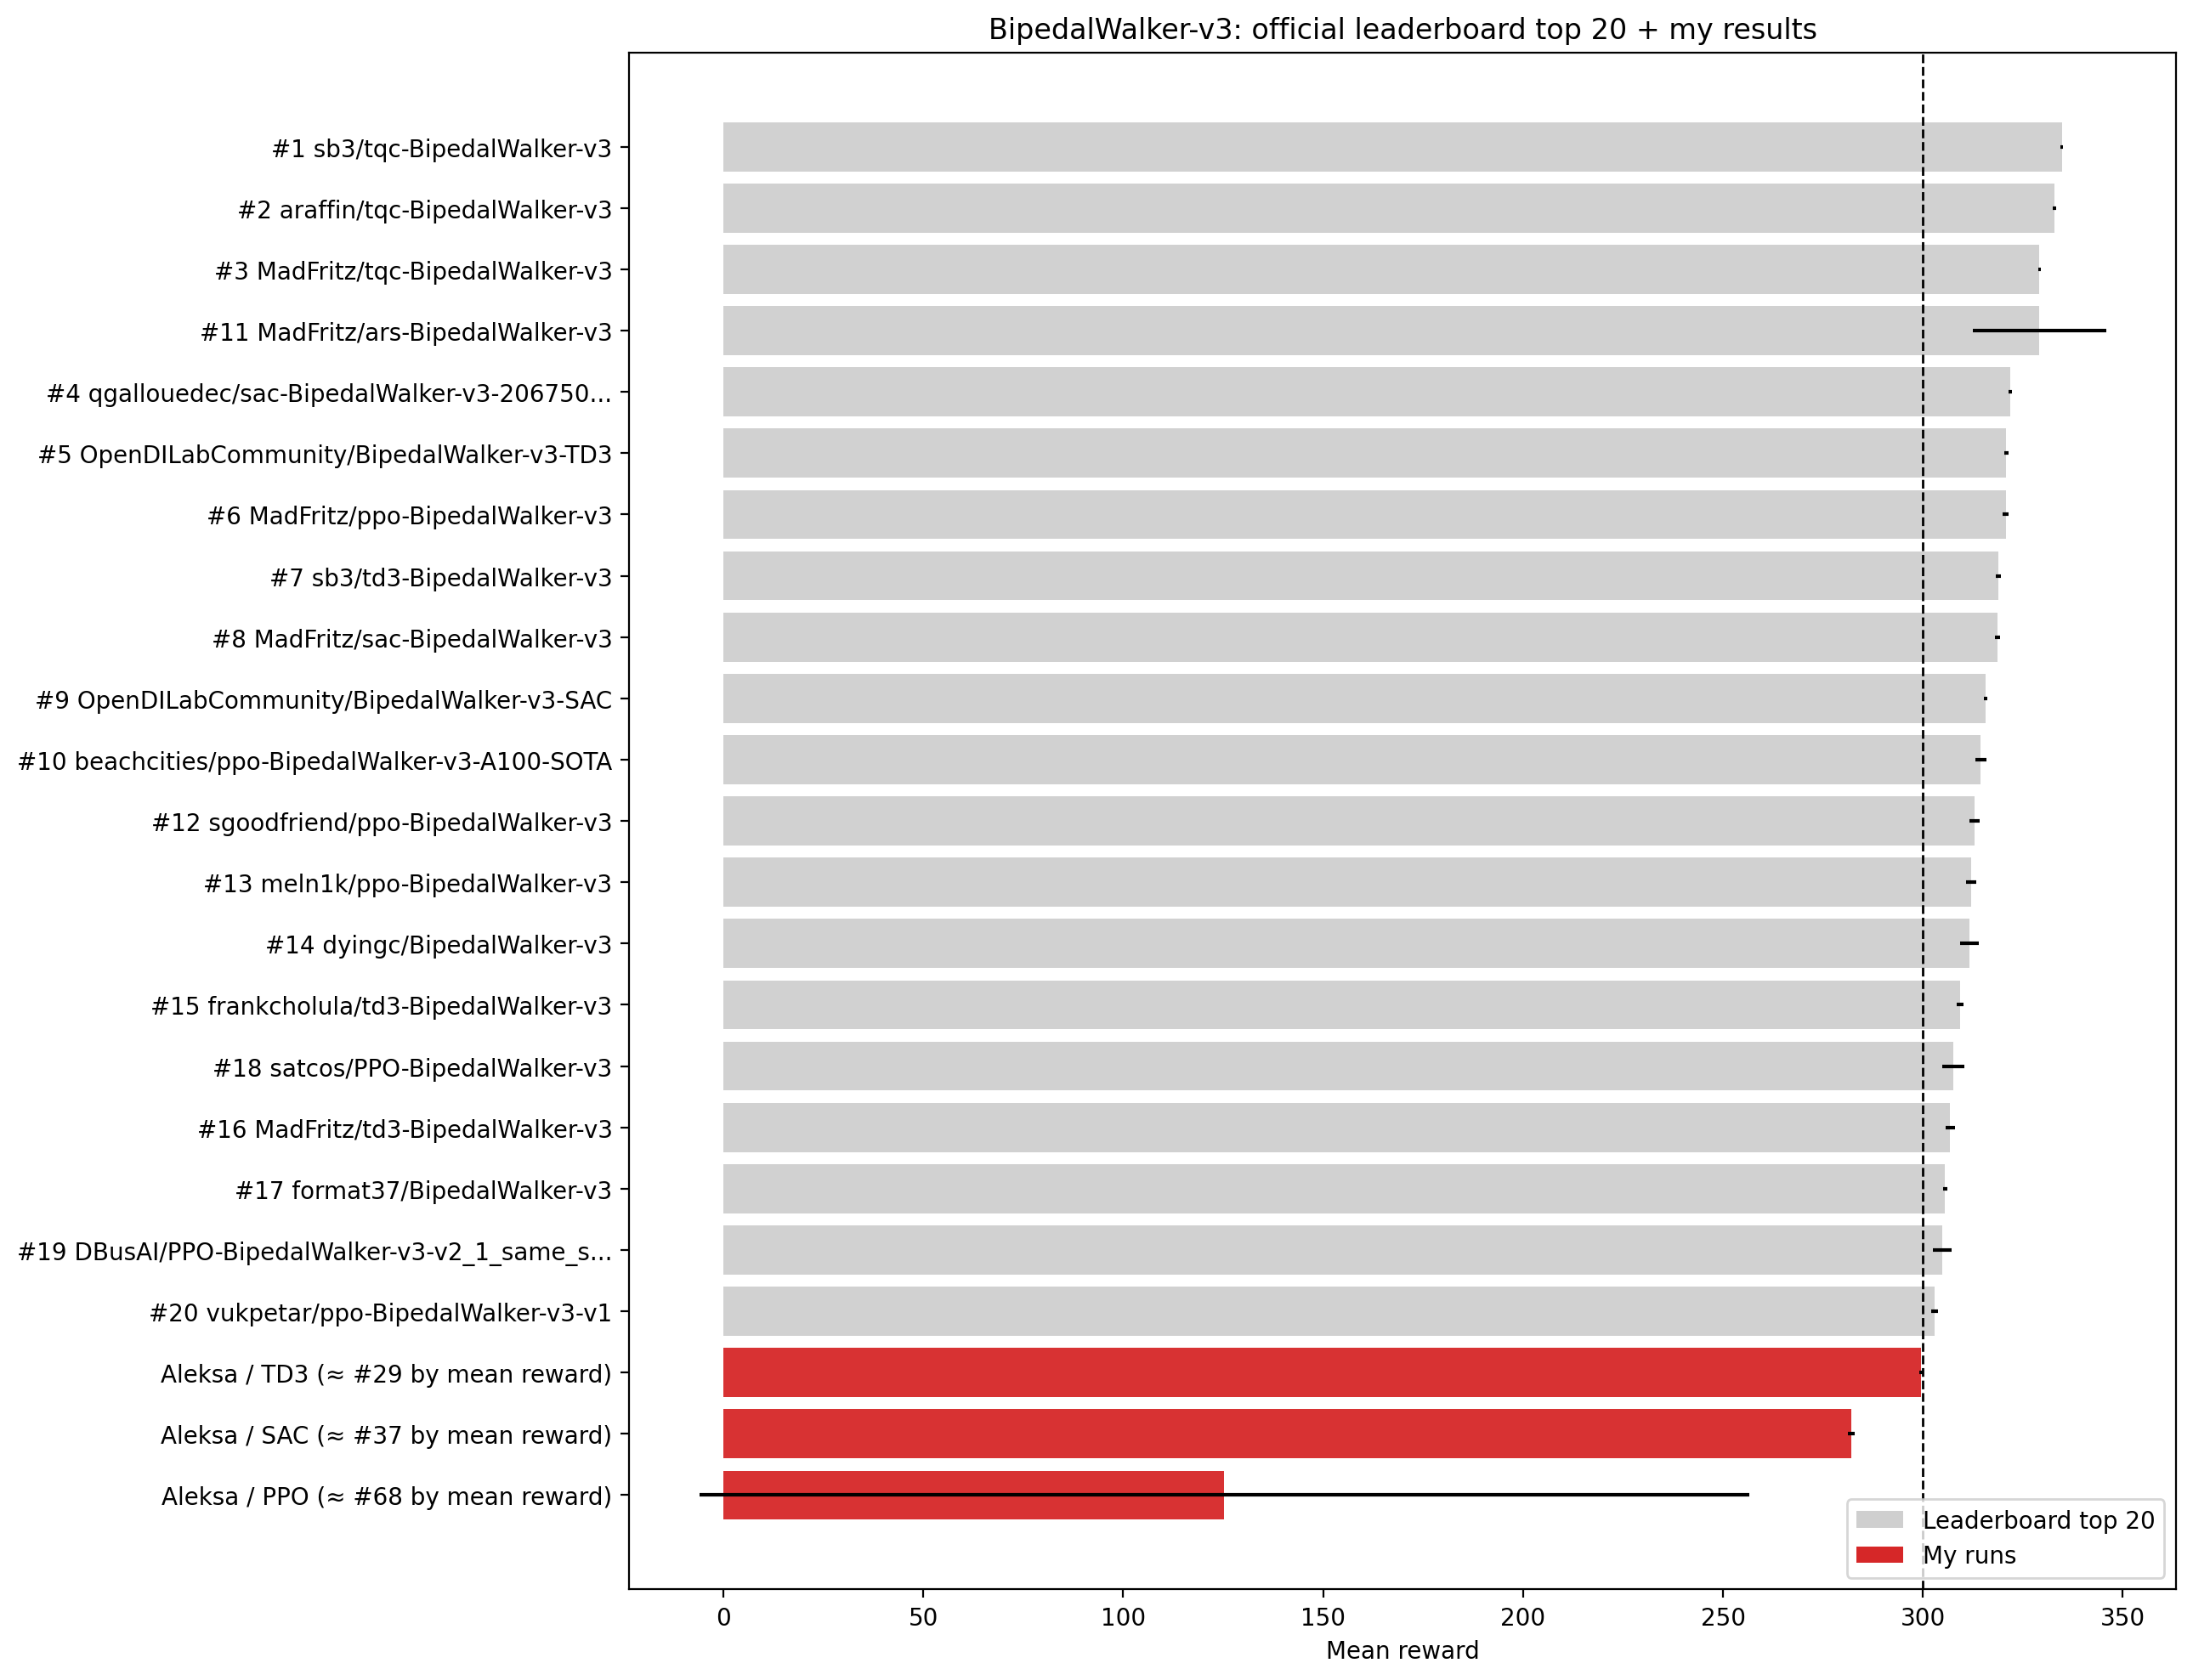
\includegraphics[width=.94\textwidth]{bipedalwalker_top20_vs_me.png}
\caption{Poređenje na standardnom zadatku. Gore: PPO, SAC i TD3 iz ovog
rada naspram odgovarajućih SB3 referentnih modela. Dole: prvih 20 javnih
prijava i približan položaj modela iz ovog rada prema srednjoj nagradi.
Različiti protokoli treninga i evaluacije ograničavaju direktno
rangiranje.}
\label{fig:standard-rewards}
\end{figure}

\subsection{Polazni modeli na hardcore okruženju}

\begin{table}[H]
\centering
\caption{Polazni modeli na hardcore zadatku.}
\begin{tabularx}{\textwidth}{lrrrY}
\toprule
Model & Budžet & \(n\) & Nagrada & Tumačenje \\
\midrule
Nasumična politika & -- & 5 & \(-109,56\pm8,08\) & Donja referentna vrednost. \\
PPO & 100\,000\,000 & 5 & \(-98,81\pm20,90\) &
Rezultat ostaje nizak, uz česte rane padove. \\
TD3 & 300\,000 & 5 & \(-116,88\pm24,80\) &
Svih pet epizoda dostiže 2000 koraka, ali bez značajnog napretka. \\
\bottomrule
\end{tabularx}
\end{table}

Dužina epizode sama po sebi nije dovoljna za procenu uspešnosti, jer TD3
u svih pet evaluacija dostiže vremensko ograničenje bez značajnog
napretka. Zbog toga su, pored numeričkih rezultata, analizirani i
odgovarajući video-snimci.

\subsection{SAC--LSTM eksperimenti}

\begin{table}[H]
\centering
\caption{Rezultati SAC--LSTM pristupa na hardcore zadatku.}
\label{tab:sac-lstm}
\begin{tabularx}{\textwidth}{YrrrY}
\toprule
Eksperiment & Koraci politike & \(n\) & Srednja sirova nagrada & Značenje \\
\midrule
Početni SAC--LSTM & 218\,923 & 1 & \(-31,64\) &
Pojedinačna evaluacija ukazuje na poboljšanje, ali nije dovoljna za
pouzdan zaključak. \\
SAC--LSTM sa mehanizmom protiv stagnacije & 927\,369 & 20 &
\(40,01\pm67,98\) &
Prva evaluacija sa pozitivnom srednjom sirovom nagradom. \\
Nastavljeni trening SAC--LSTM modela & 1\,920\,280 & 5 &
\(160,90\pm113,97\) &
Odvojena evaluacija sa sačuvanim video-snimcima. \\
Stanje modela nakon 4600 epizoda & 1\,357\,542 & 5 &
\(\mathbf{216,84\pm76,06}\) &
Najbolja sačuvana višeepizodna evaluacija za koju su dostupne
pojedinačne nagrade. \\
\bottomrule
\end{tabularx}
\end{table}

Broj koraka politike dobijen je sabiranjem stvarno zabeleženih dužina
trening epizoda, bez evaluacionih epizoda. Veličina mini-batch-a od 64 ne
množi ovaj broj, jer se uzorci za ažuriranje ponovo uzimaju iz replay
buffer-a. Uz \texttt{frame\_skip}=2, stanje nakon 4600 epizoda zato
odgovara 1\,357\,542 odluke politike i najviše 2\,715\,084 koraka simulatora.

Tokom treninga je zabeležena i periodična evaluacija sa srednjom nagradom
\(239,39\) u 20 epizoda. Kako pojedinačne nagrade i standardna devijacija
za ovu proveru nisu sačuvane, rezultat se ne koristi kao glavni rezultat
u tabeli niti kao osnova za poređenje varijabilnosti.

Za najbolju sačuvanu višeepizodnu evaluaciju stanja modela nakon 4600 epizoda
pojedinačne sirove nagrade su \(291,39\), \(197,40\), \(217,92\),
\(292,21\) i \(85,28\). Slika~\ref{fig:best-eval} pokazuje da dve epizode dostižu rezultat
blizak granici od 300 poena, dok razlika između epizoda ukazuje na
osetljivost politike na konkretan raspored terena.

\begin{figure}[H]
\centering
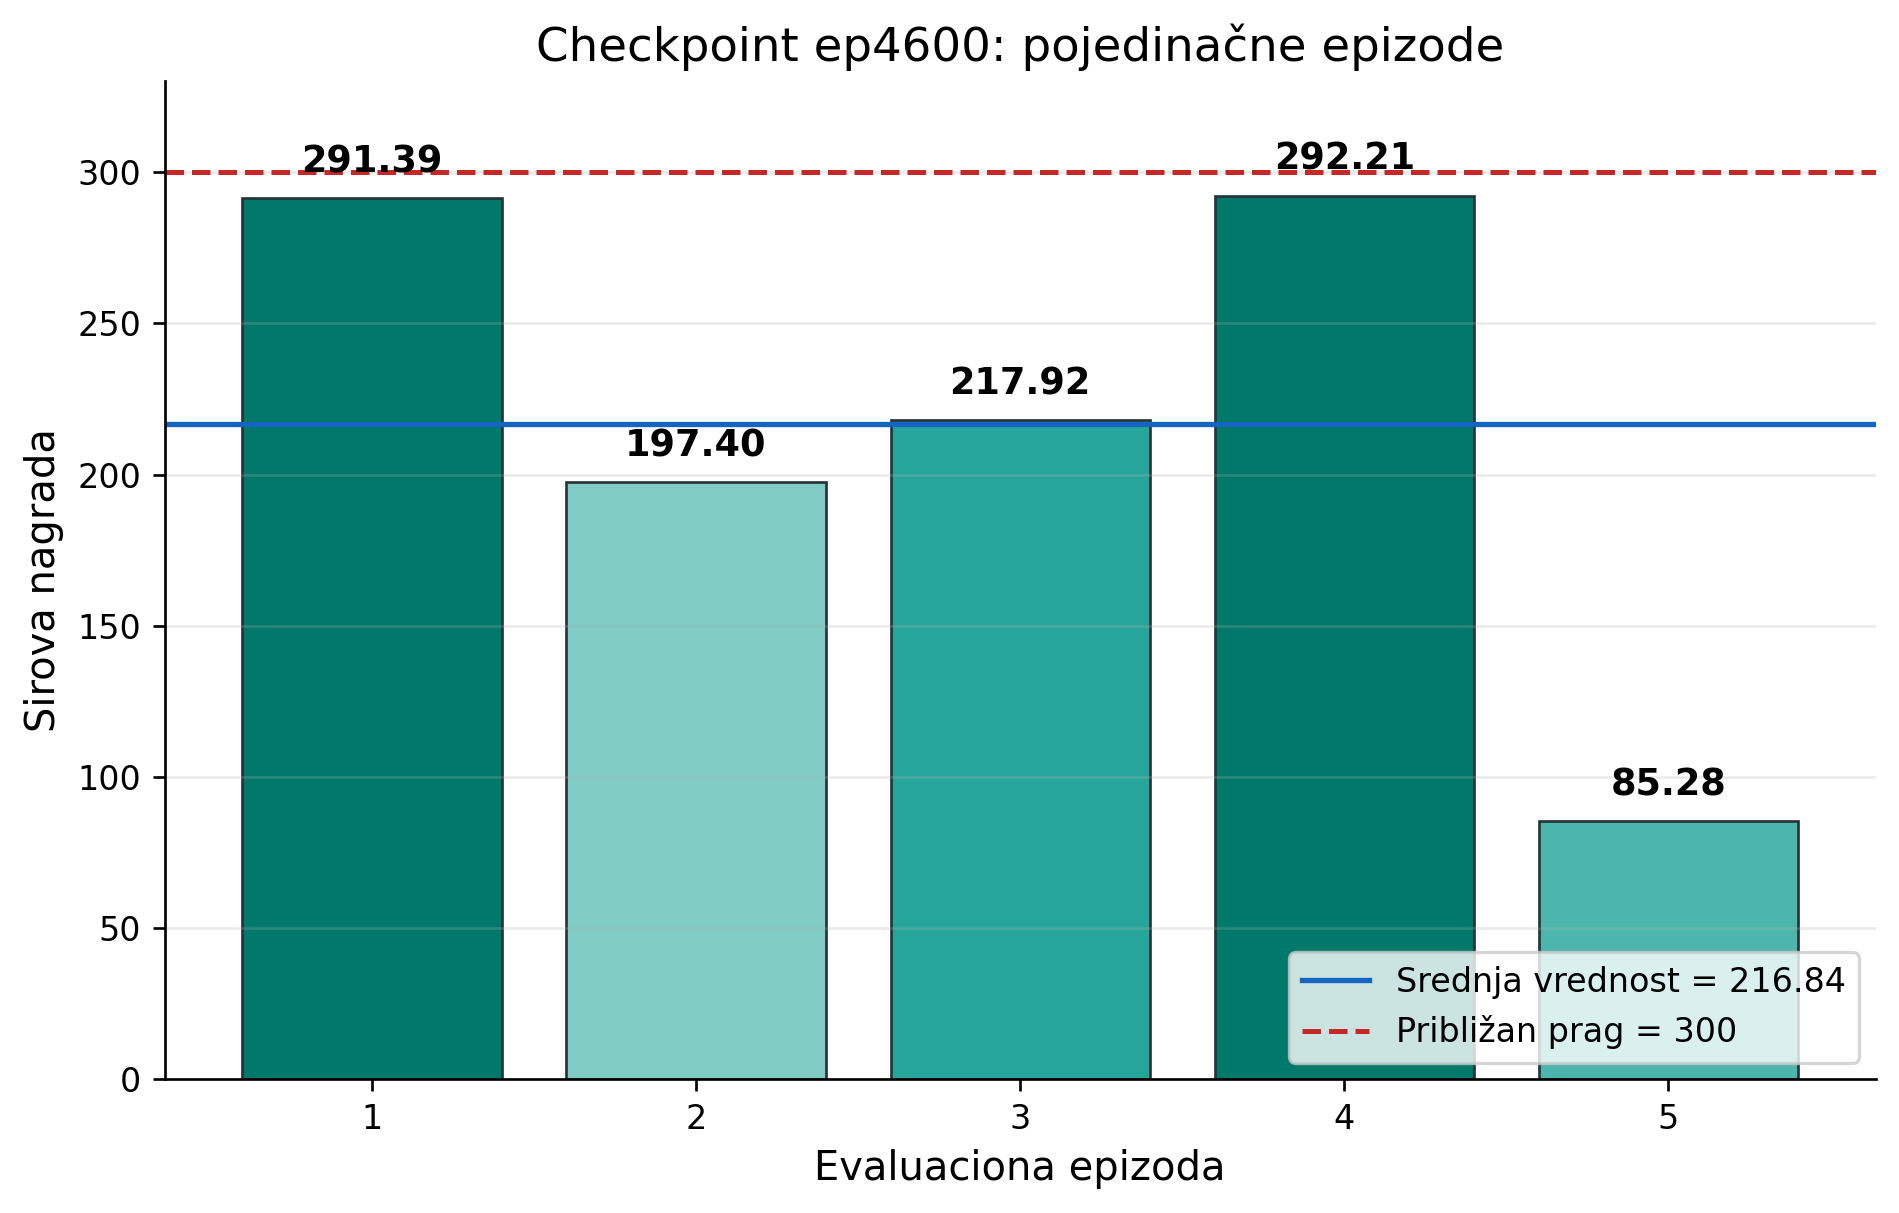
\includegraphics[width=.90\textwidth]{best_evaluation_episodes.png}
\caption{Pojedinačne sirove nagrade stanja modela nakon 4600 epizoda.
Dve evaluacije ostvaruju rezultat blizak 300 poena, ali razlika među
epizodama pokazuje da politika još nije dovoljno stabilna.}
\label{fig:best-eval}
\end{figure}

\begin{figure}[H]
\centering
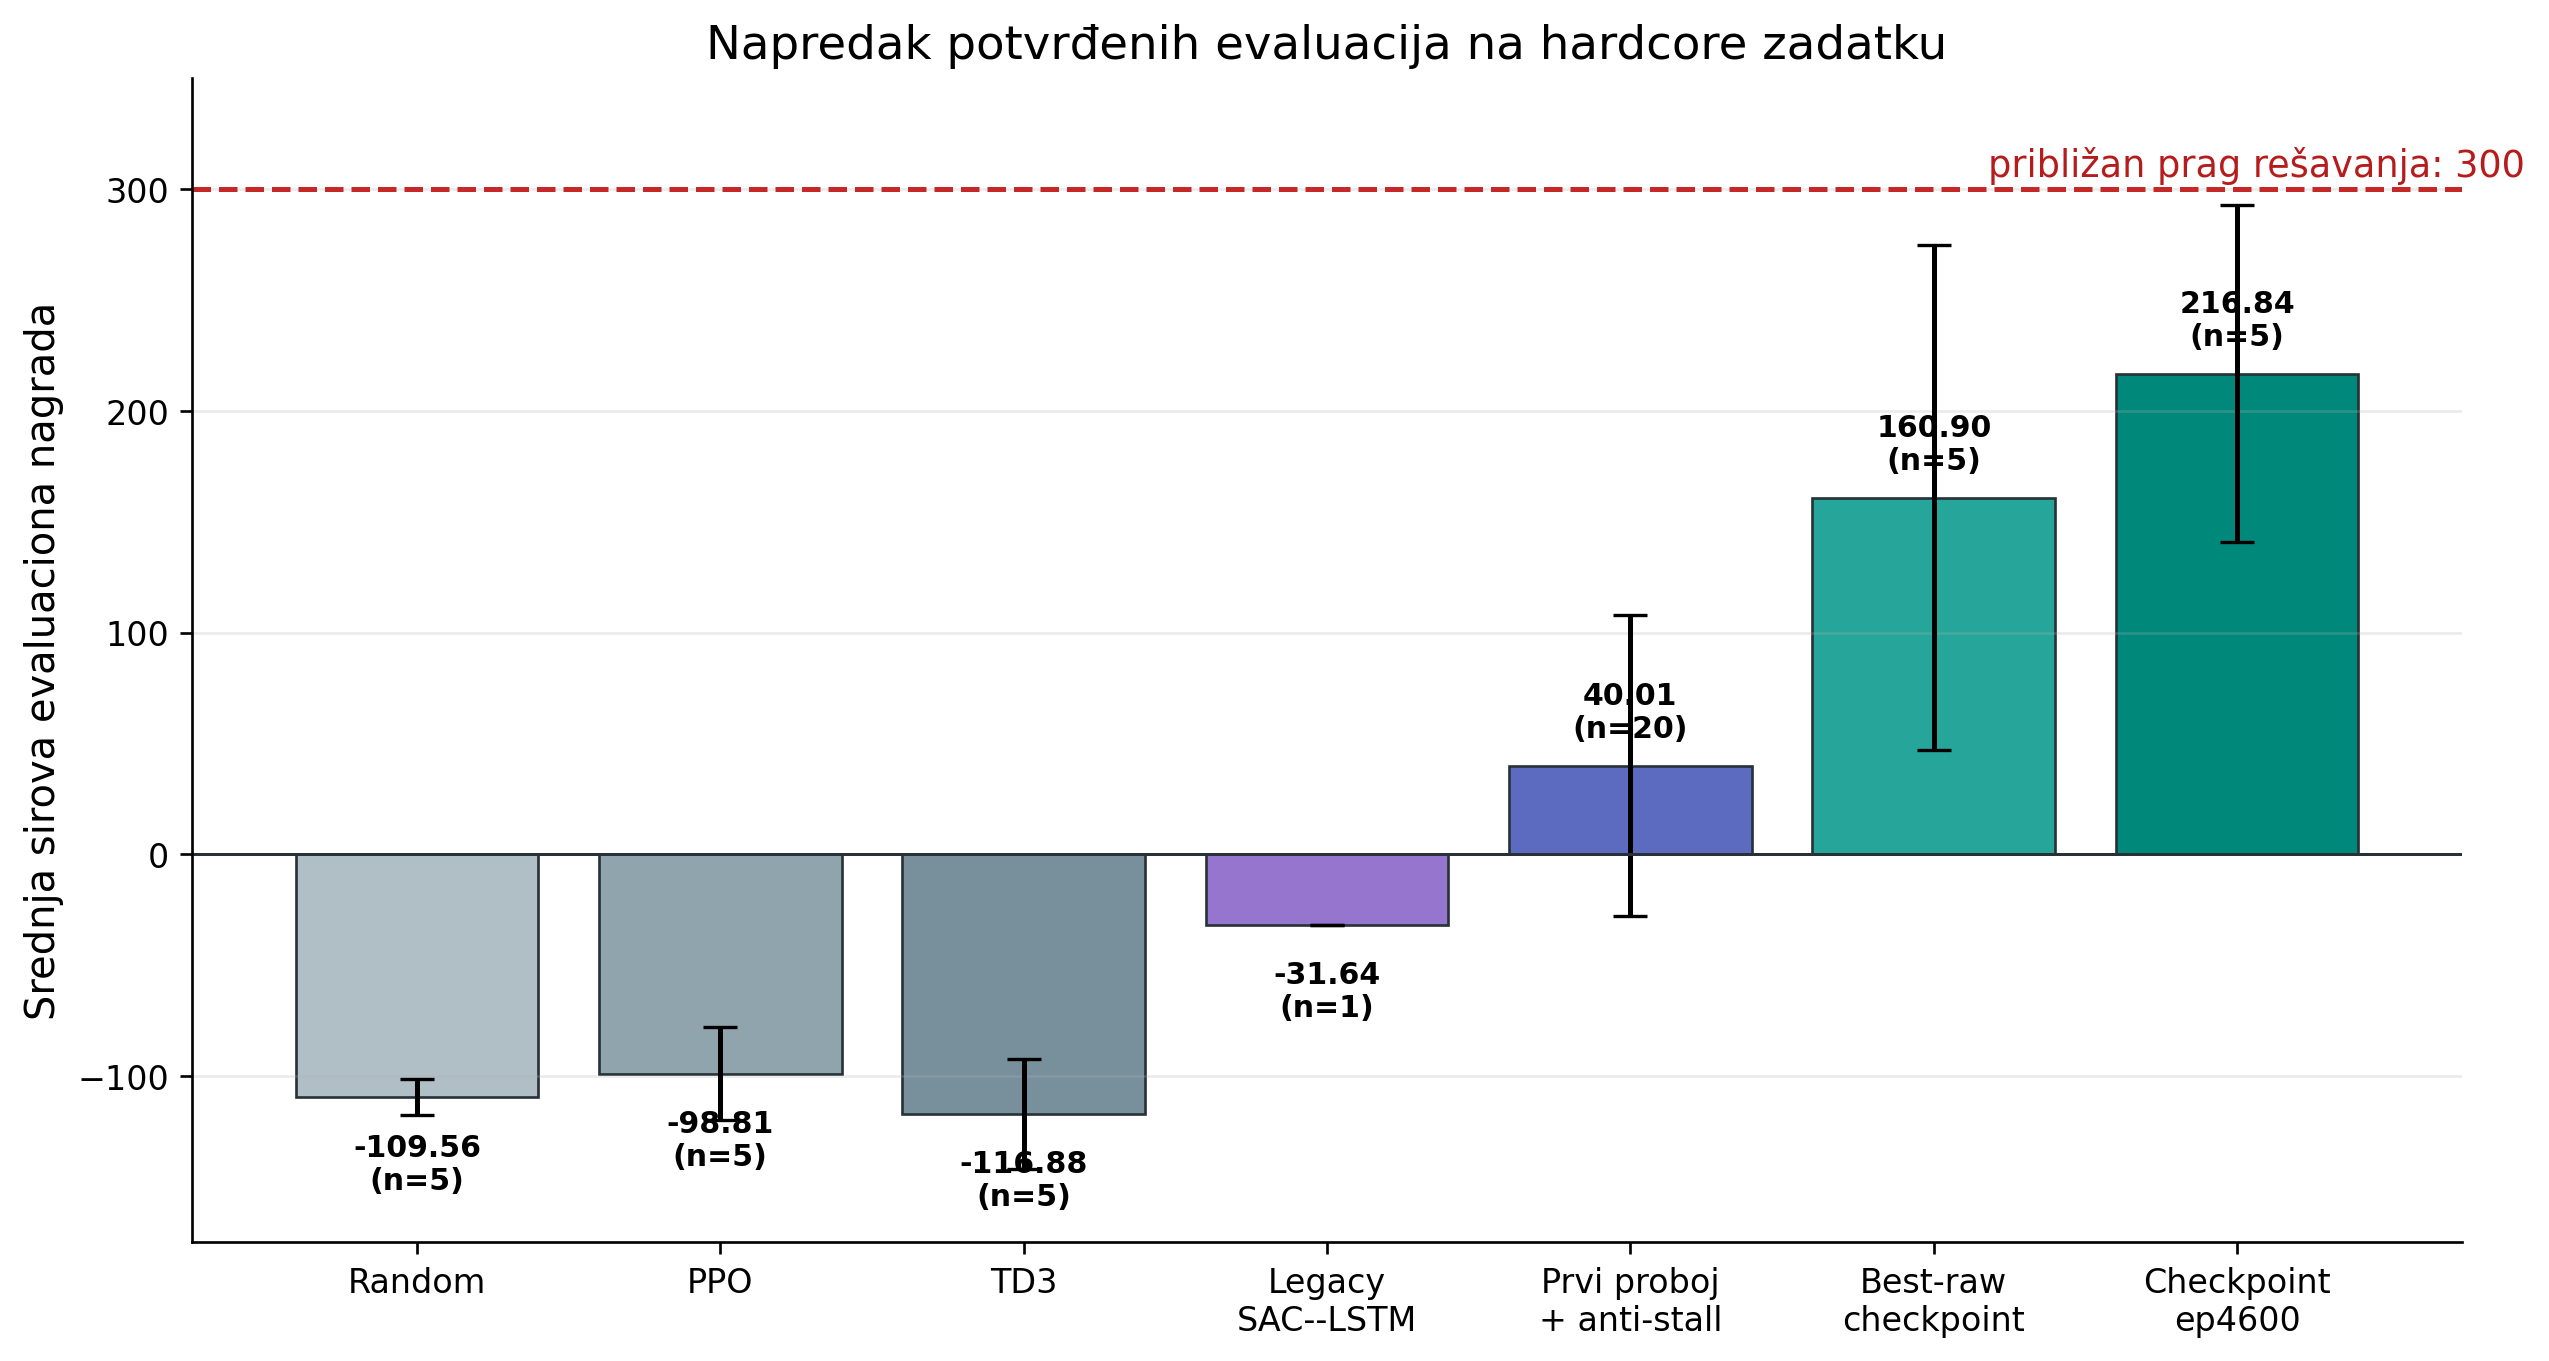
\includegraphics[width=.94\textwidth]{hardcore_model_progression.png}
\caption{Razvoj sačuvanih višeepizodnih evaluacija na hardcore zadatku.
Vertikalne linije predstavljaju standardnu devijaciju, a \(n\) broj
evaluacionih epizoda. Periodični rezultat \(239,39\) nije prikazan kao
ravnopravan rezultat jer nisu sačuvane pojedinačne nagrade.}
\label{fig:hardcore-progression}
\end{figure}

Na Slici~\ref{fig:hardcore-progression} prikazane su evaluacije za koje
su dostupni broj epizoda i standardna devijacija.

Sačuvani logovi omogućavaju i prikaz promene nagrade tokom treninga.
Slika~\ref{fig:training-curve} prikazuje početni trening do epizode 3200
i njegov nastavak iz sačuvanog stanja modela. X-osa prikazuje kumulativne
korake politike. Zbog podešavanja \texttt{frame\_skip}=2, jedan korak
politike obuhvata do dva koraka simulatora.

\begin{figure}[H]
\centering
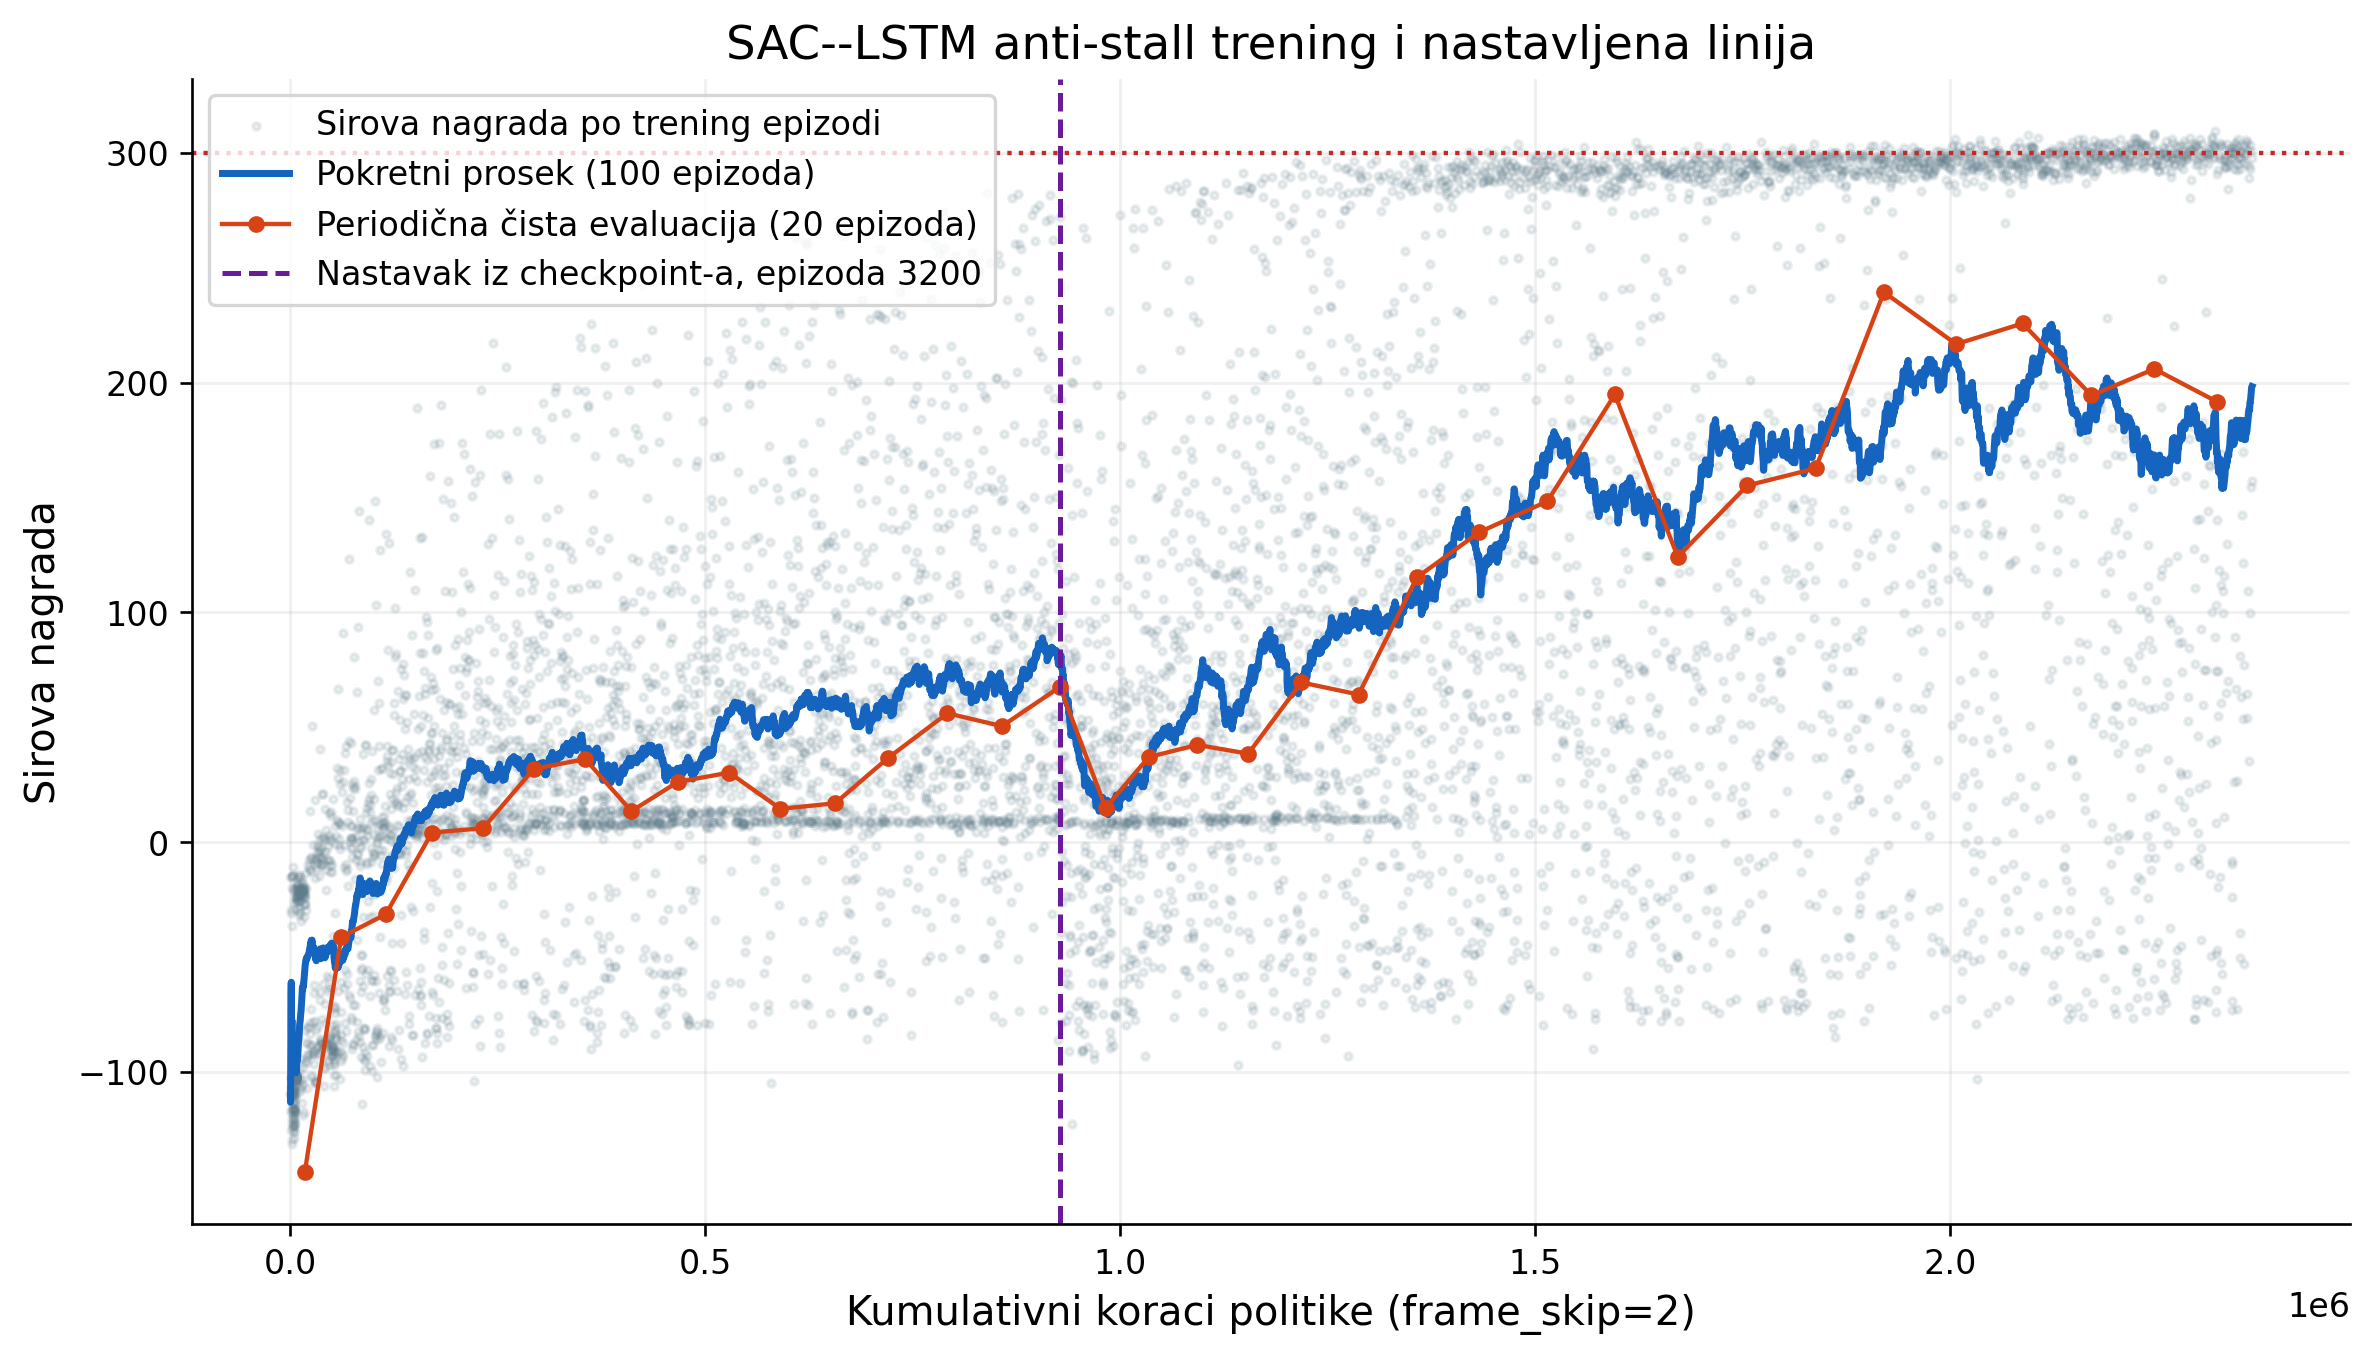
\includegraphics[width=.96\textwidth]{training_curve_sac_lstm.png}
\caption{Sirova nagrada tokom treninga, pokretni prosek od 100 epizoda
i periodične evaluacije SAC--LSTM modela. Vertikalna linija označava
nastavak treninga iz stanja sačuvanog nakon epizode 3200.}
\label{fig:training-curve}
\end{figure}

\section{Analiza grešaka}

Najvažniji uočeni režimi neuspeha su:
\begin{itemize}
  \item \textbf{rani pad} --- PPO često gubi ravnotežu pre ostvarenog
  značajnijeg napretka;
  \item \textbf{stagnacija} --- TD3 može ostati uspravan do vremenskog
  ograničenja bez uspešnog savladavanja prepreka;
  \item \textbf{lokalni optimum} --- javljaju se stabilni obrasci
  oscilovanja koji ne dovode do napretka;
  \item \textbf{osetljivost na teren} --- SAC--LSTM u nekim evaluacijama
  prolazi veći deo staze, dok u drugim rano prestaje da napreduje;
  \item \textbf{razlika između sirove i oblikovane nagrade} --- dodatne
  kazne i prekidi pomažu tokom treninga, zbog čega se konačni zaključci
  zasnivaju na originalnoj nagradi okruženja.
\end{itemize}

Video-snimci daju direktnu kvalitativnu potvrdu tri različita režima
ponašanja (Slika~\ref{fig:failure-modes}). Izabrani kadrovi vezani su za
konkretne JSON evaluacije i semena.

\begin{figure}[H]
\centering
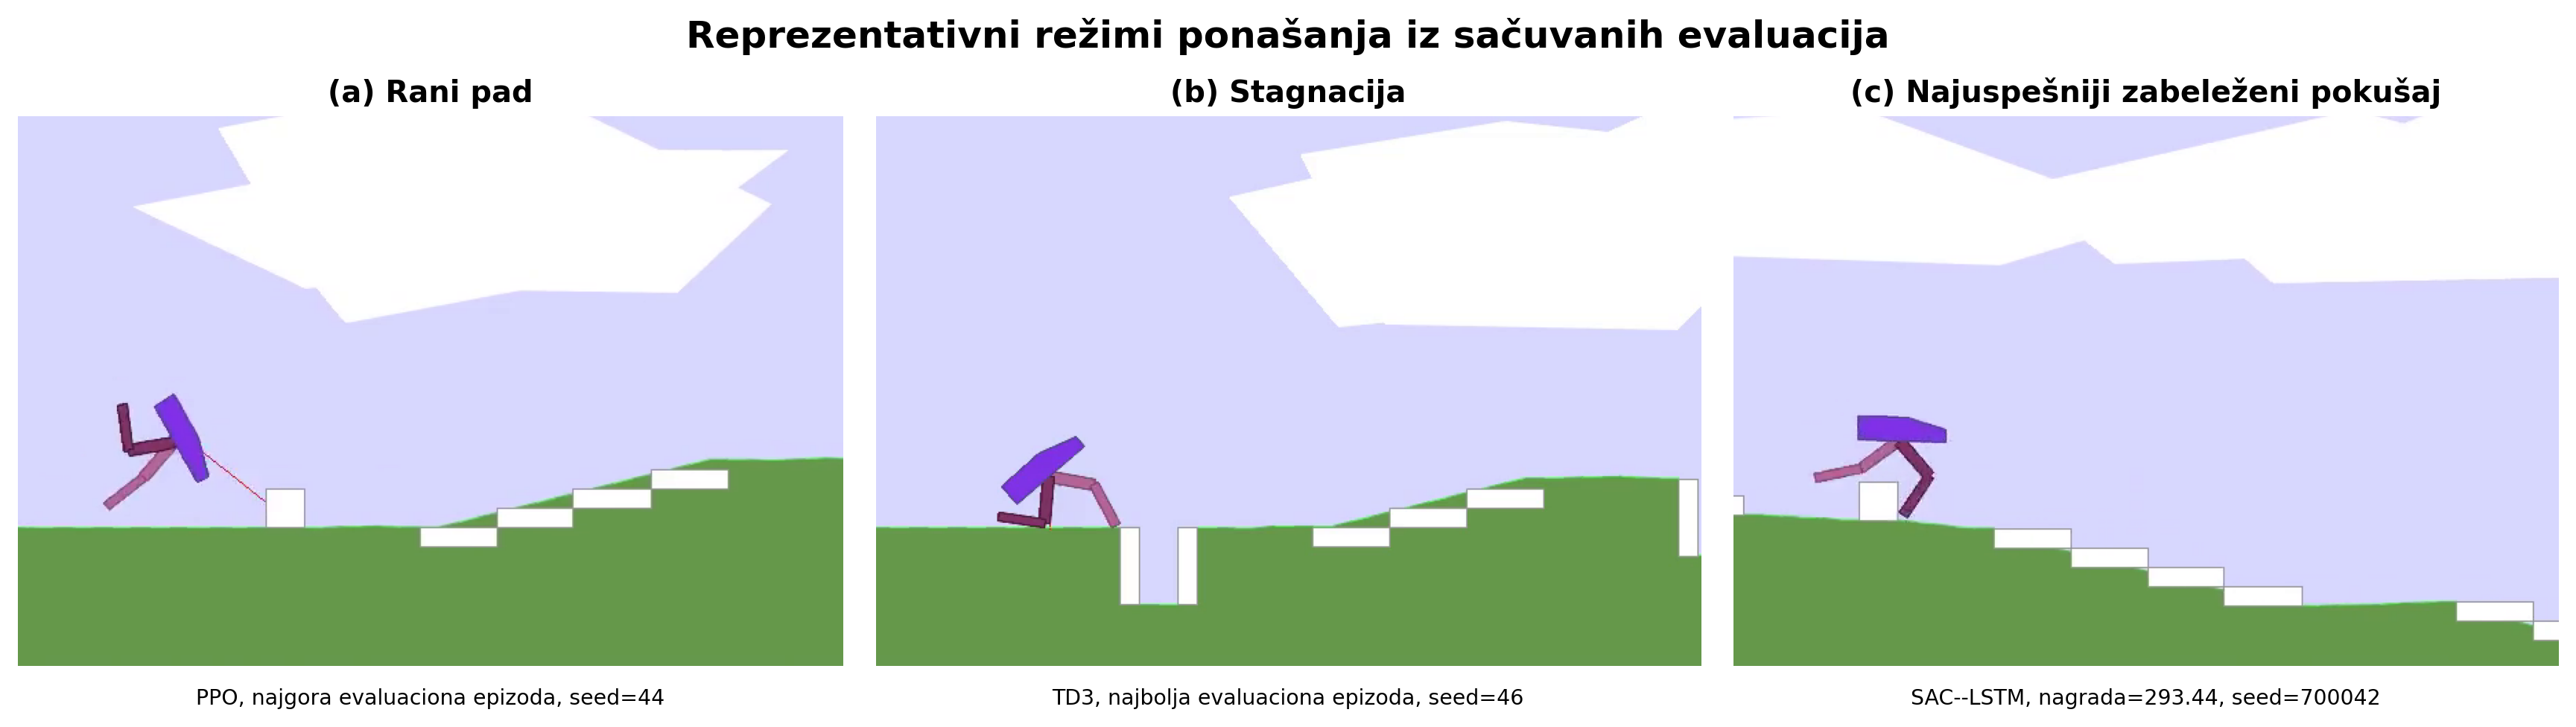
\includegraphics[width=\textwidth]{failure_modes.png}
\caption{Reprezentativni kadrovi iz sačuvanih evaluacija: (a) PPO,
najgora epizoda za seme 44, neposredno pre ranog pada; (b) TD3,
najbolja epizoda za seme 46, u kojoj agent ostaje kod prve jame do
vremenskog limita; (c) SAC--LSTM, seme 700042 i sirova nagrada
\(293,44\), nakon prolaska preko više prepreka. Poslednji primer je
skoro uspešna, ali ne formalno rešena epizoda.}
\label{fig:failure-modes}
\end{figure}

Rani pad PPO agenta ukazuje na nedovoljno stabilnu kontrolu ravnoteže.
Kod TD3 agenta položaj se gotovo ne menja između 15. i 30. sekunde
snimka, što pokazuje zašto dužina epizode od 2000 koraka nije dokaz
napretka. SAC--LSTM kadar potvrđuje delimično korisnu politiku za
prelazak prepreka, ali raspodela nagrada na
Slici~\ref{fig:best-eval} pokazuje da ta strategija nije dovoljno
robusna između evaluacionih semena.

Mehanizam za sprečavanje stagnacije direktno utiče na epizode u kojima
agent ne ostvaruje horizontalni napredak, dok LSTM omogućava da odluka
zavisi od kratke istorije kretanja. Nakon uvođenja ovih izmena prvi put
je dobijena pozitivna srednja sirova nagrada u višeepizodnoj evaluaciji.
Ipak, bez kontrolisanog ablacionog eksperimenta na više nezavisnih
trening semena nije moguće precizno izdvojiti doprinos svake komponente.

\section{Poređenje sa javno prijavljenim rezultatima}

Pored međusobnog poređenja obučenih modela, rezultate je korisno
posmatrati i u odnosu na javne prijave na OpenAI Gym leaderboard-u
\cite{gymleaderboard}. Za hardcore zadatak prag rešavanja iznosi prosečno
300 poena tokom 100 uzastopnih epizoda. Zbog toga jedna epizoda sa
nagradom bliskom 300 ne predstavlja dokaz da je zadatak stabilno rešen.
Leaderboard sadrži rezultate za verzije \texttt{v2} i \texttt{v3}, ali one
nisu potpuno ekvivalentne zbog izmene lidar opservacija u verziji
\texttt{v3}. Slika~\ref{fig:hardcore-leaderboard} zato koristi samo javne
prijave za verziju korišćenu u ovom radu.

\begin{figure}[H]
\centering
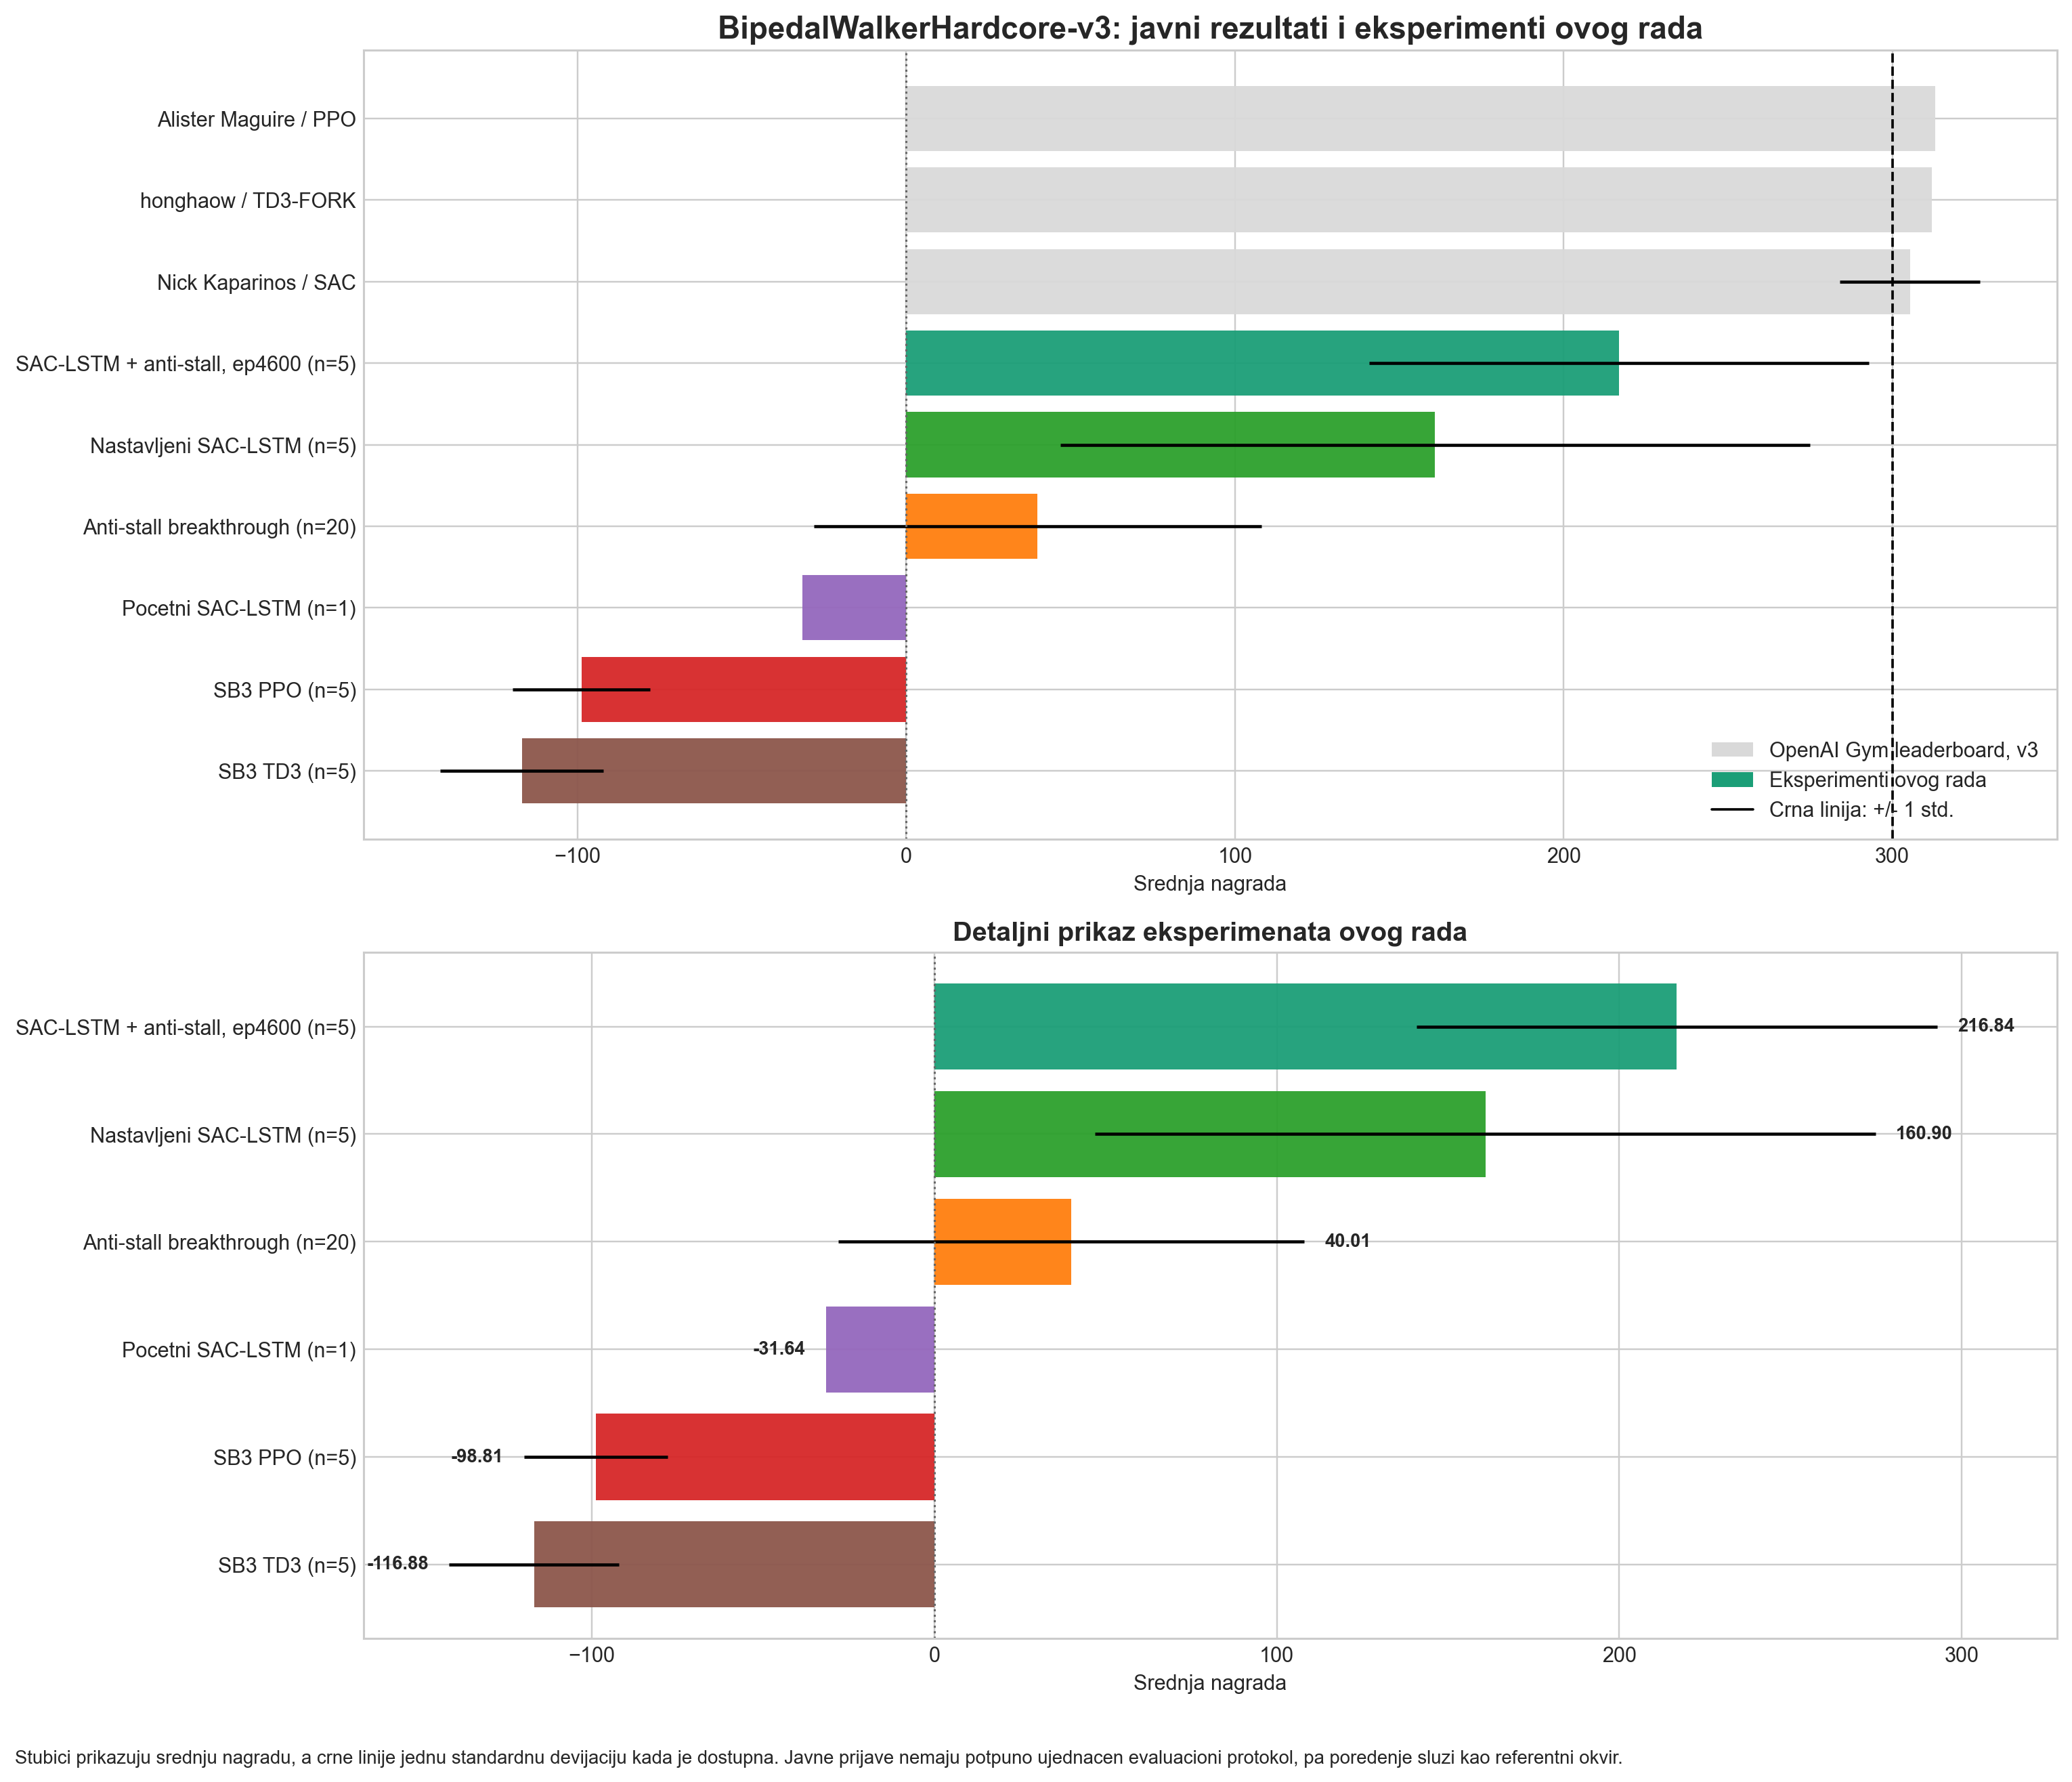
\includegraphics[width=.96\textwidth]{hardcore_vs_leaderboard_reference.png}
\caption{Izabrani javno prijavljeni rezultati za
\texttt{BipedalWalkerHardcore-v3} i eksperimenti ovog rada. Crne linije
predstavljaju jednu standardnu devijaciju kada je dostupna. Glavni
rezultat ovog rada je stanje nakon 4600 epizoda sa
\(216,84\pm76,06\) u pet evaluacionih epizoda.}
\label{fig:hardcore-leaderboard}
\end{figure}

Prikazani javni rezultati pokazuju da se zadatak može rešiti različitim
porodicama algoritama: on-policy PPO pristupom \cite{ppo}, off-policy SAC
pristupom \cite{sac}, kao i TD3 varijantom proširenom forward-looking
mehanizmom. Prema tome, rekurentna memorija nije neophodan uslov za
rešavanje okruženja. U ovom radu LSTM ima drugačiju ulogu: modelu daje
kratak vremenski kontekst, dok mehanizam protiv stagnacije smanjuje broj
epizoda u kojima agent ostaje kod prepreke bez napretka.

Najbolja sačuvana višeepizodna evaluacija ovog rada,
\(216,84\pm76,06\), niža je od javno prijavljenih proseka iznad 300.
Dve od pet epizoda ostvaruju 291,39 i 292,21 poena, što potvrđuje da je
naučeno korisno ponašanje, ali velika standardna devijacija pokazuje da
ono nije dovoljno robusno za različite konfiguracije terena. Rezultat se
zato tumači kao parcijalno naučena politika, a ne kao rešen hardcore
zadatak.

Direktno rangiranje ipak bi bilo metodološki nepouzdano. Model ovog rada
evaluiran je u pet epizoda, dok formalni kriterijum zahteva 100, a za deo
leaderboard prijava potpun evaluacioni protokol nije naveden. Ni broj
trening epizoda nije potpuna mera budžeta: stanje modela nakon 4600
epizoda odgovara 1\,357\,542 koraka politike, dok za javne prijave nisu
dosledno dostupni broj koraka, \texttt{frame\_skip} i drugi detalji.
Leaderboard zato služi kao referentni okvir za procenu preostalog jaza,
a ne kao strogo kontrolisan eksperiment.

\section{Zaključak i dalji rad}

Na standardnom \texttt{BipedalWalker-v3} zadatku najbolji prijavljeni
rezultat ostvaruje TD3 sa srednjom nagradom \(299,54\), dok SAC postiže
nešto niži, ali veoma stabilan rezultat. Prenos standardnih pristupa na
\texttt{BipedalWalkerHardcore-v3} pokazao se znatno zahtevnijim: PPO
ostvaruje niske nagrade uz česte padove, dok TD3 može da ostane uspravan
do vremenskog ograničenja bez značajnog napretka.

Uvođenjem istorije od 12 opservacija, LSTM enkodera i mehanizma za
sprečavanje stagnacije dobijeno je jasno poboljšanje. Najbolja sačuvana
višeepizodna evaluacija ostvaruje \(216,84\pm76,06\), pri čemu dve od pet
epizoda dostižu rezultat blizak 300 poena. Ipak, velika razlika između
pojedinačnih epizoda pokazuje da politika još nije dovoljno robusna da bi
se hardcore zadatak smatrao stabilno rešenim.

Za dalji rad potrebno je ponoviti trening sa više nezavisnih seed-ova,
izjednačiti budžet interakcija između modela i sve modele evaluirati na
istom skupu test semena. Posebno je značajno sprovesti ablaciono
poređenje modela bez LSTM komponente, bez mehanizma protiv stagnacije i
sa obe komponente, kako bi se izdvojio njihov pojedinačni doprinos.
Pored srednje nagrade i standardne devijacije, korisno je pratiti procenat
epizoda sa rezultatom većim ili jednakim 300, kao i prepreke na kojima se
agent najčešće zaustavlja.


\begin{thebibliography}{9}

\bibitem{gymnasium}
Farama Foundation,
\emph{Bipedal Walker --- Gymnasium Documentation}.
\url{https://gymnasium.farama.org/environments/box2d/bipedal_walker/}

\bibitem{ppo}
J. Schulman, F. Wolski, P. Dhariwal, A. Radford i O. Klimov,
\emph{Proximal Policy Optimization Algorithms}, 2017.
\url{https://arxiv.org/abs/1707.06347}

\bibitem{sac}
T. Haarnoja, A. Zhou, P. Abbeel i S. Levine,
\emph{Soft Actor-Critic: Off-Policy Maximum Entropy Deep Reinforcement
Learning with a Stochastic Actor}, ICML, 2018.
\url{https://proceedings.mlr.press/v80/haarnoja18b.html}

\bibitem{td3}
S. Fujimoto, H. van Hoof i D. Meger,
\emph{Addressing Function Approximation Error in Actor-Critic Methods},
ICML, 2018.
\url{https://proceedings.mlr.press/v80/fujimoto18a.html}

\bibitem{sb3}
A. Raffin et al.,
\emph{Stable-Baselines3: Reliable Reinforcement Learning
Implementations}, JMLR, 2021.
\url{https://www.jmlr.org/papers/v22/20-1364.html}

\bibitem{gymleaderboard}
OpenAI Gym,
\emph{Leaderboard}, GitHub Wiki.
\url{https://github.com/openai/gym/wiki/Leaderboard}

\bibitem{hfleaderboard}
Hugging Face,
\emph{Deep Reinforcement Learning Course Leaderboard Data:
BipedalWalker-v3}.
\url{https://huggingface.co/datasets/huggingface-projects/drlc-leaderboard-data}

\end{thebibliography}


\end{document}
